\section*{Chapter 6: Backpropagation}

\subsection*{Layers}

Activation:
$\mathbf z_l = F_{l:1}(\mathbf x) = F_l(\mathbf z_{l-1})$

Map
$F: \R^n \rightarrow \R^m$

$\partial_{ij}F=\partial_iF_j:\R^n\rightarrow\R$

Jacobian
$\partial F=\partial_{ji}F:\R^n\rightarrow\R^{m\times n}$

$\partial F=\prod^1_{l=k}\partial F_l\circ F_{l-1:1}$ 

or $\partial F(\mathbf x)=\prod^1_{l=k}\partial F_l(\mathbf z_{l-1})$

\textbf{Layered DNN gradient} (without loss):

$\nabla_{\mathbf \theta_l}F=(\partial F_{k:l+1}\circ F_{l:1})\cdot (F'_l\circ F_{l-1:1})$ or

$\nabla_{\mathbf \theta_l}F(\mathbf x)=\partial F_{k:l+1}(\mathbf z_l)\cdot F'_l(\mathbf z_{l-1})$

\textbf{Backpropagation} (w/ loss $\ell$, $f=\ell\circ F$):

$\nabla_{\mathbf \theta_l}f(\mathbf x)=\partial (\ell \circ F_{k:l+1})(\mathbf z_l)\cdot F'_l(\mathbf z_{l-1})$
where 

$\xi_l = \partial (\ell \circ F_{k:l+1})(\mathbf z_l)$ can be computed through the backward iteration:

$\xi_k = \partial l(\mathbf z_k), \xi_{l-1} = \xi_l \partial F_l(\mathbf z_{l-1})$

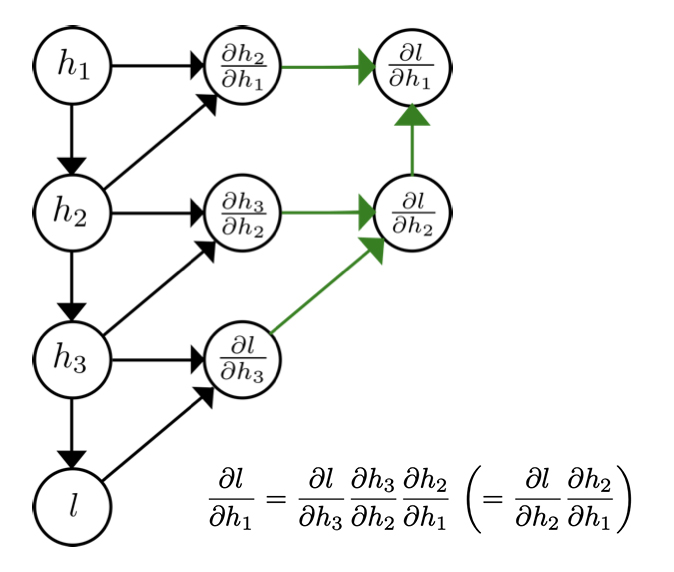
\includegraphics[width=0.7\columnwidth]{src/comp-graph.jpg}
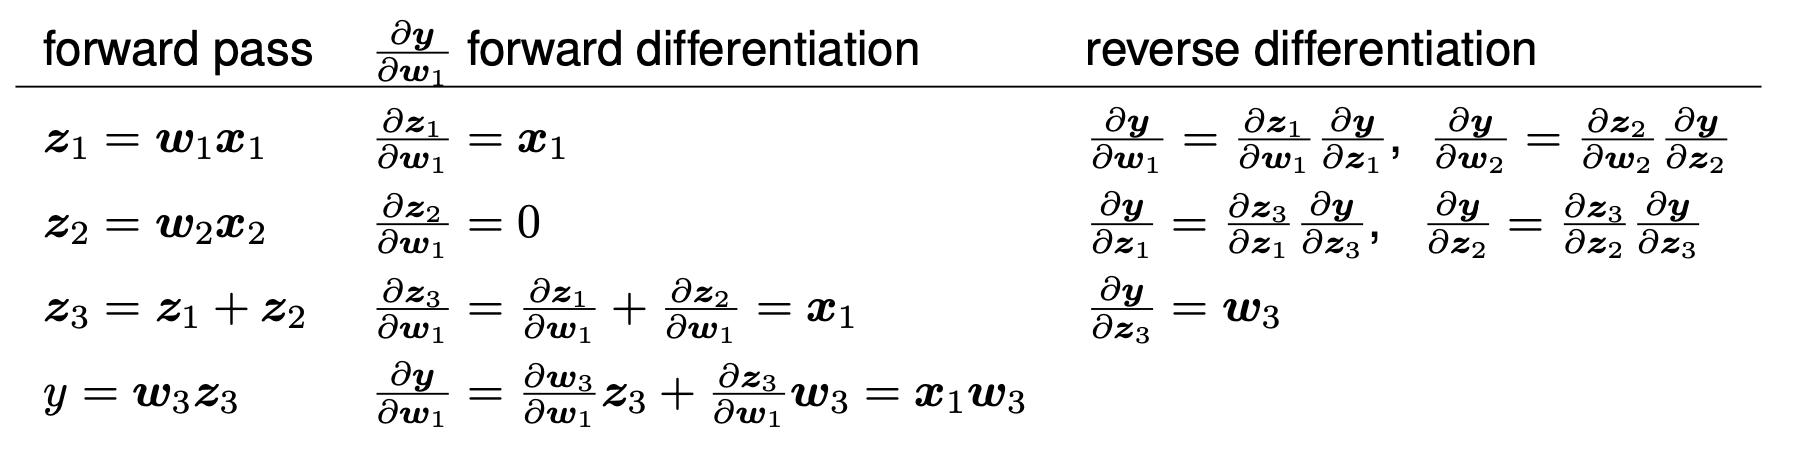
\includegraphics[width=\columnwidth]{src/diff-modes.png}

Forward prop: $O(\#params)$

Backward prop: $O(\#outputs)$